\section{Experiment}
\subsection{Simulation Settings}
\begin{frame}
  \frametitle{Experiment Settings}
  \only<1>{
    Hardware
    \begin{itemize}
      \item Intel Core i5 3570 (2C4T)
      \item 16GB RAM
      \item Ubuntu 14.04 LTS
      \item Ruby 2.1.1
    \end{itemize}
  }

  \only<2>{
    Sleep-based simulation
    \begin{itemize}
      \item Sample from obtained data center logs.
      \item Take allocated CPUs as task amount and assign random numbers
        as job priorities.
      \item Sleep according to the execution time.
      \item 20 worker instances used.
    \end{itemize}
  }

  \only<3>{
    Homogeneous Environment
    \begin{itemize}
      \item Tasks in a job has identical sleep time.
      \item Each worker simply sleeps the time hold by that task.
    \end{itemize}

    Heterogeneous Environment
    \begin{itemize}

      \item Each worker will sleep an randomized additional period
        related to a worker parameter.
      \item Specify different parameter to represent different computing
        speed.
      \item Pick 1/20 of the task as GPU task and 4 out of 20 workers as
        GPU server.  When GPU task is send to a GPU worker, its sleep
        time is reduced to 1/10.
    \end{itemize}

  }
\end{frame}

\subsection{Homogeneous}
\begin{frame}
  \frametitle{Experiment Results --- Homogeneous}
  \begin{figure}[htbp]
    \centering
    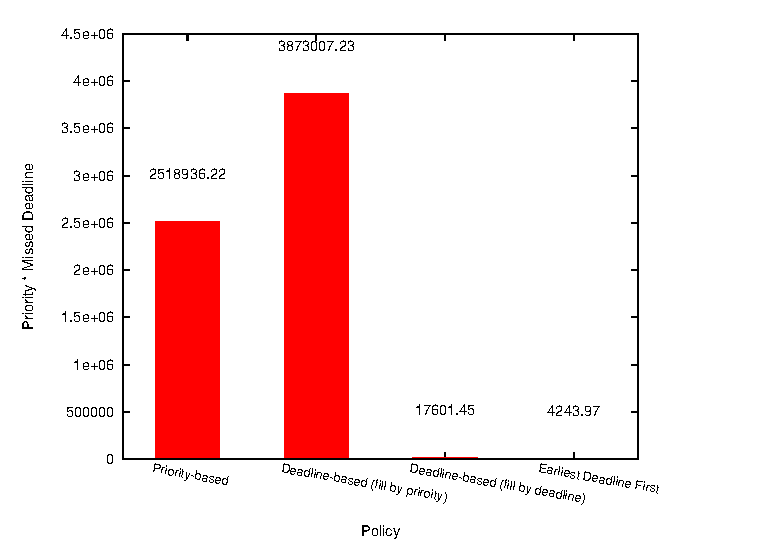
\includegraphics[width=\textwidth,height=0.7\textheight,keepaspectratio]{figures/homo.eps}
    \caption{Homogeneous Environment Setting}
  \end{figure}
\end{frame}

